\documentclass[11pt]{amsart}
\usepackage[margin=1in]{geometry}
\usepackage{amsmath,amssymb,mathtools}
\usepackage{graphicx}
\usepackage{xcolor}
\usepackage{hyperref}
\hypersetup{colorlinks=true,linkcolor=blue!55!black,citecolor=blue!55!black,urlcolor=blue!55!black}
\emergencystretch=2em

\newtheorem{theorem}{Theorem}
\newtheorem{proposition}[theorem]{Proposition}
\newtheorem{lemma}[theorem]{Lemma}
\newtheorem{corollary}[theorem]{Corollary}
\theoremstyle{definition}
\newtheorem{remark}[theorem]{Remark}

\newcommand{\Leb}{\mathcal L}
\newcommand{\Borel}{\mathcal B}
\newcommand{\Cp}{C_p}
\newcommand{\Np}{N^{1,p}}

\title[Borel representatives can fail]{A complete snowflake counterexample to the\
Borel-representative problem for Newtonian functions}
\author{Literature-implied answer packet for arXiv:1509.02326}
\date{13 August 2026}

\begin{document}

\begin{abstract}
Bj\"orn--Bj\"orn--Mal\'y asked whether every bounded Newtonian function on a metric
space with a positive complete Borel measure finite on balls has a Borel
representative.  We give a negative answer for every $1\le p<\infty$.
Snowflake the interval by $d_\alpha(x,y)=|x-y|^\alpha$, $0<\alpha<1$, and
equip it with an explicit complete finite non-Borel-regular extension of
Lebesgue measure.  There are no nonconstant rectifiable curves, so
$\Np=L^p$ and $\Cp(E)=\mu(E)$ for measurable $E$.  The characteristic
function of a Bernstein set then has no Borel representative.  More
generally, on this snowflaked interval all Newtonian functions have Borel
representatives if and only if the measure is Borel regular, by a 2024
theorem of Alvarado--Gorka--Slabuszewski.  We classify the result as
literature-implied because that theorem supplies the general regularity
criterion, although it does not mention the Newtonian problem.
\end{abstract}

\maketitle

\noindent
\fbox{\parbox{0.94\textwidth}{\textbf{Status.}
Literature-implied full negative answer, with an explicit construction and
complete proof supplied for human review.}}

\section{The source problem and the later criterion}

The source is A.~Bj\"orn, J.~Bj\"orn, and J.~Mal\'y,
\emph{Quasiopen and $p$-path open sets, and characterizations of
quasicontinuity}, arXiv:1509.02326~\cite{source}.  Under the standing
assumptions $1\le p<\infty$ and a metric space carrying a positive complete
Borel measure finite on balls, their Open Problem 5.3 asks:

\begin{center}

\includegraphics[width=0.96\textwidth]{figures/source_problem.png}

\small Source evidence: Open Problem 5.3, PDF page 13 of arXiv:1509.02326.
\end{center}

Here a representative of $u\in\Np(X)$ means a function equal to $u$
quasieverywhere, with respect to the source's Sobolev capacity.

A later theorem supplies the measure-theoretic dividing line.  In
arXiv:2410.21434, Alvarado--Gorka--Slabuszewski prove that, for a metric space
with a nonnegative measure defined on a sigma-algebra containing the Borel
sets and finite on balls, the following are equivalent: the measure is Borel
regular, and every measurable function has a Borel representative
almost everywhere~\cite{support}.

\begin{center}
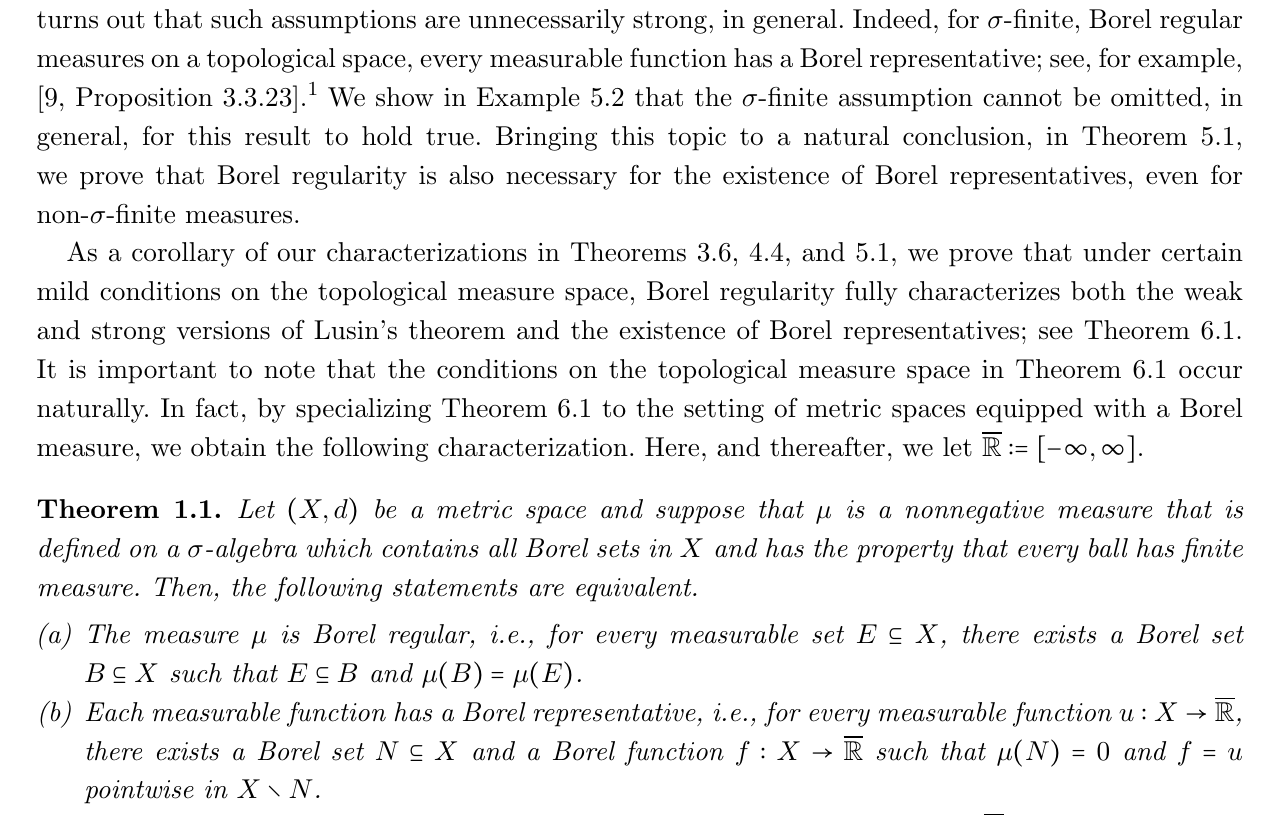
\includegraphics[width=0.98\textwidth]{figures/support_theorem.png}

\small Supporting evidence: Theorem 1.1(a)--(b), PDF page 2 of
arXiv:2410.21434.
\end{center}

That paper does not cite the source problem and does not discuss Newtonian
spaces.  The reduction below makes its relevance exact and also gives a fully
explicit witness.

\section{The snowflake reduction}

Fix $0<\alpha<1$ and put
\[
 X=[0,1],\qquad d_\alpha(x,y)=|x-y|^\alpha.
\]
This metric induces the usual topology.  Thus $X$ is compact, complete, and
separable, and its Borel sets are the usual Borel subsets of the interval.

\begin{lemma}\label{lem:no-curves}
There is no nonconstant rectifiable curve in $(X,d_\alpha)$.
\end{lemma}

\begin{proof}
Let $\gamma:[a,b]\to X$ be continuous and nonconstant.  Choose $s<t$ such
that $\gamma(s)\ne\gamma(t)$, reverse the parameter if necessary, and write
$x=\gamma(s)<y=\gamma(t)$ and $L=y-x>0$.  For an integer $n\ge1$, continuity
and the intermediate value theorem give successive first hitting times
\[
 s=t_0<t_1<\cdots<t_n\le t,
 \qquad \gamma(t_j)=x+\frac{jL}{n}.
\]
The $d_\alpha$-length of $\gamma$ is therefore at least
\[
 \sum_{j=1}^n d_\alpha(\gamma(t_{j-1}),\gamma(t_j))
 =n\left(\frac Ln\right)^\alpha
 =L^\alpha n^{1-\alpha}.
\]
This tends to infinity, so $\gamma$ is not rectifiable.
\end{proof}

Let $\mu$ be any complete finite Borel measure on this space, in the source's
sense that its domain sigma-algebra contains all Borel sets.  Because upper
gradients in the source are tested on nonconstant compact rectifiable curves,
Lemma~\ref{lem:no-curves} makes the zero function an upper gradient of every
measurable function.

\begin{proposition}\label{prop:collapse}
For every $1\le p<\infty$,
\[
 \Np(X)=L^p(X,\mu),\qquad
 \|f\|_{\Np}=\|f\|_{L^p}.
\]
Moreover, for every measurable $E\subseteq X$,
\[
 \Cp(E)=\mu(E).
\]
Consequently two measurable Newtonian functions agree quasieverywhere if and
only if they agree almost everywhere.
\end{proposition}

\begin{proof}
The first assertion follows immediately from the zero upper gradient and the
definition of the Newtonian norm.  If $h\in\Np(X)$ satisfies $h\ge1$ on
$E$, then
\[
 \|h\|_{\Np}^p=\int_X|h|^p\,d\mu\ge\mu(E),
\]
so $\Cp(E)\ge\mu(E)$.  Conversely $h=\mathbf1_E$ is measurable, lies in
$L^p$ because $\mu$ is finite, has upper gradient zero, and is admissible;
hence $\Cp(E)\le\mu(E)$.  The last assertion follows by applying the identity
to the measurable discrepancy set.
\end{proof}

In particular, the later Borel-regularity theorem immediately yields the
following sharp statement for this reduction class.

\begin{corollary}\label{cor:iff}
On the snowflaked interval above, every function in $\Np(X)$ has a Borel
representative for every $1\le p<\infty$ if and only if $\mu$ is Borel
regular.
\end{corollary}

\begin{proof}
If $\mu$ is Borel regular, Theorem 1.1 of~\cite{support} gives a Borel
almost-everywhere representative of every measurable $L^p$ function, and
Proposition~\ref{prop:collapse} upgrades almost-everywhere equality to
quasieverywhere equality.  Conversely, if every Newtonian function has a
Borel representative, then every bounded measurable function does, because
$\mu(X)<\infty$ and $\Np=L^p$.  In particular every characteristic function
has a Borel representative; equivalently, one may apply the implication from
Borel representatives to Borel regularity in~\cite{support}.
\end{proof}

\section{An explicit complete nonregular measure}

We now construct the promised measure rather than merely invoking the
existence of a non-Borel-regular one.  Recall that a \emph{Bernstein set}
$A\subseteq[0,1]$ is a set such that both $A$ and $A^c$ meet every nonempty
perfect subset of $[0,1]$.  Such sets exist by the classical transfinite
construction: enumerate the nonempty perfect sets and choose two fresh
points from each, putting one into $A$ and reserving the other for $A^c$.

Neither $A$ nor $A^c$ contains a Lebesgue-measurable set of positive measure.
Indeed, every positive-measure Lebesgue set contains a nonempty perfect set,
which would contradict one of the two defining intersection properties.
Thus
\begin{equation}\label{eq:innerzero}
 \lambda_*(A)=\lambda_*(A^c)=0.
\end{equation}

Let $\Leb$ be the Lebesgue sigma-algebra and define
\[
 \Sigma=
 \bigl\{(B\cap A)\cup(C\cap A^c):B,C\in\Leb\bigr\}.
\]
This is a sigma-algebra: complements and countable unions are computed
coordinatewise on $A$ and $A^c$.  It contains $\Leb$, because
$D=(D\cap A)\cup(D\cap A^c)$ for every $D\in\Leb$.  Define
\begin{equation}\label{eq:mu}
 \mu\bigl((B\cap A)\cup(C\cap A^c)\bigr)
 =\frac{\lambda(B)+\lambda(C)}2.
\end{equation}

\begin{lemma}\label{lem:measure}
Formula~\eqref{eq:mu} is well-defined and gives a complete probability
measure on $\Sigma$.  Its restriction to $\Leb$ is Lebesgue measure.
\end{lemma}

\begin{proof}
Suppose two pairs $(B,C)$ and $(B',C')$ represent the same set.  Then
$B\mathbin\triangle B'\subseteq A^c$ and
$C\mathbin\triangle C'\subseteq A$.  These symmetric differences are
Lebesgue measurable, so~\eqref{eq:innerzero} says that both are null.  The
right side of~\eqref{eq:mu} is therefore independent of the representation.

For countable additivity, let represented sets $E_n$ be pairwise disjoint,
with coordinates $(B_n,C_n)$.  For $n\ne m$, the measurable intersection
$B_n\cap B_m$ is contained in $A^c$, and $C_n\cap C_m$ is contained in $A$.
Both intersections are null by~\eqref{eq:innerzero}.  Thus each coordinate
family is pairwise disjoint modulo null sets, and Lebesgue countable
additivity applied to the coordinatewise union proves countable additivity
of $\mu$.

If $E=(B\cap A)\cup(C\cap A^c)$ is $\mu$-null, then $B$ and $C$ are
Lebesgue null.  Every subset of $E$ splits into a subset of $B\cap A$ and a
subset of $C\cap A^c$; these two subsets are Lebesgue measurable by
completeness of Lebesgue measure and hence give a member of $\Sigma$.
Therefore $\mu$ is complete.  Finally, a Lebesgue set $D$ has the
representation $(B,C)=(D,D)$, so $\mu(D)=\lambda(D)$.  In particular
$\mu(X)=1$.
\end{proof}

This $\mu$ is a positive complete Borel measure finite on balls: it contains
the usual Borel sigma-algebra, agrees there with Lebesgue measure, and every
nonempty open ball has positive finite measure.  It is not Borel regular.
Indeed, $\mu(A)=1/2$, while every Borel $D\supseteq A$ has
$D^c\subseteq A^c$.  By~\eqref{eq:innerzero}, $\lambda(D^c)=0$, whence
$\mu(D)=\lambda(D)=1$.

The same computation gives the stronger identity
\begin{equation}\label{eq:distance}
 \mu(A\mathbin\triangle D)
 =\frac{\lambda(D^c)+\lambda(D)}2=\frac12
 \qquad\text{for every Borel }D\subseteq X.
\end{equation}

\section{The full negative answer}

\begin{theorem}\label{thm:main}
For every $1\le p<\infty$ there is a compact complete metric space $X$ with
a finite positive complete Borel measure $\mu$, and a bounded function
$u\in\Np(X)$, such that $u$ has no Borel representative.  Hence the answer
to Open Problem 5.3 of arXiv:1509.02326 is negative, even simultaneously for
all finite $p$ on one metric measure space.
\end{theorem}

\begin{proof}
Use the snowflaked interval and the measure of
Lemma~\ref{lem:measure}, and put $u=\mathbf1_A$.  This function is bounded
and measurable.  Since $\mu(X)=1$, Proposition~\ref{prop:collapse} gives
$u\in\Np(X)$ for every finite $p$.

Suppose a Borel function $v$ represented $u$.  The Borel set
$D=\{x:v(x)>1/2\}$ would satisfy
\[
 \{u\ne v\}\supseteq A\mathbin\triangle D.
\]
In particular~\eqref{eq:distance} gives
$\mu(\{u\ne v\})\ge1/2$.  Proposition~\ref{prop:collapse} then yields
\[
 \Cp(\{u\ne v\})=\mu(\{u\ne v\})\ge\frac12>0,
\]
contradicting equality quasieverywhere.  Thus no Borel representative exists.
\end{proof}

\begin{remark}[Provenance]
Theorem~\ref{thm:main} is filed as a literature-implied answer, not as a
novel counterexample.  The general equivalence between Borel regularity and
Borel representatives is already Theorem 1.1 of~\cite{support}; the
snowflake collapse, explicit Bernstein-set extension, and connection to the
2015 Newtonian open problem are supplied here.  The supporting paper contains
no citation to the source paper and no occurrence of ``Newtonian'' or
``quasiopen,'' so it does not appear to advertise this consequence.
\end{remark}

\begin{thebibliography}{9}

\bibitem{source}
A.~Bj\"orn, J.~Bj\"orn, and J.~Mal\'y,
\emph{Quasiopen and $p$-path open sets, and characterizations of
quasicontinuity},
Nonlinear Analysis 138 (2016), 224--237; arXiv:1509.02326.

\bibitem{support}
R.~Alvarado, P.~G\'orka, and A.~S\l abuszewski,
\emph{Borel regularity is equivalent to Lusin's theorem and the existence of
Borel representatives},
arXiv:2410.21434 (2024).

\end{thebibliography}

\end{document}
